% Generated by tools/analysis/analyze.py; do not edit by hand.
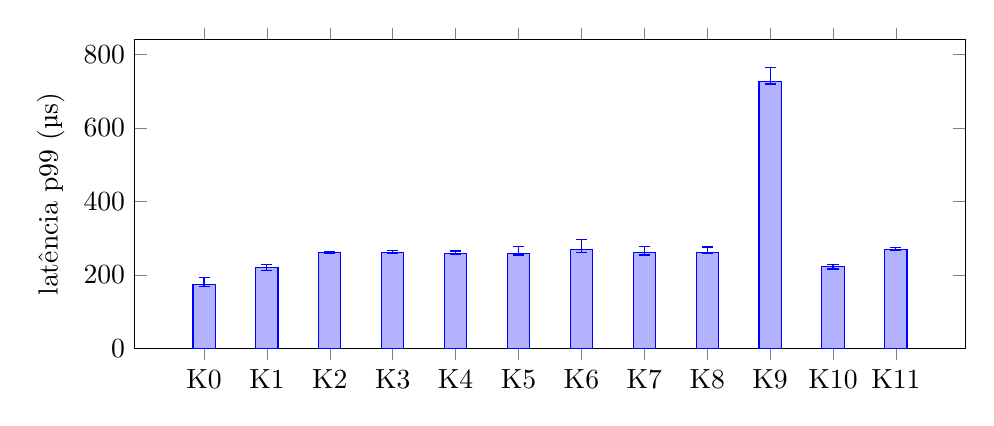
\begin{tikzpicture}
  \begin{axis}[width=\linewidth, height=5.5cm, ybar, bar width=8pt,
      ylabel={latência p99 (µs)}, xtick={0,...,11},
      xticklabels={K0,K1,K2,K3,K4,K5,K6,K7,K8,K9,K10,K11}, ymin=0,
      error bars/y dir=both, error bars/y explicit]
    \addplot+[error bars/.cd, y dir=both, y explicit] coordinates {
      (0,173.000) +- (0,0) -= (0,5.000) += (0,20.000)
      (1,220.000) +- (0,0) -= (0,9.000) += (0,9.000)
      (2,260.500) +- (0,0) -= (0,3.000) += (0,2.500)
      (3,262.000) +- (0,0) -= (0,4.000) += (0,5.500)
      (4,257.000) +- (0,0) -= (0,2.000) += (0,8.000)
      (5,258.000) +- (0,0) -= (0,4.000) += (0,19.500)
      (6,268.000) +- (0,0) -= (0,8.000) += (0,29.000)
      (7,260.500) +- (0,0) -= (0,6.500) += (0,16.000)
      (8,262.000) +- (0,0) -= (0,4.500) += (0,14.000)
      (9,725.500) +- (0,0) -= (0,5.500) += (0,38.500)
      (10,224.000) +- (0,0) -= (0,8.000) += (0,5.000)
      (11,268.500) +- (0,0) -= (0,2.500) += (0,5.500)
    };
  \end{axis}
\end{tikzpicture}
